\documentclass[systemskiss/skiss.tex]{subfiles}

\begin{document}
\section{Kommunikationsmodul}
Kommunikationsmodulen är en modul som ska kommunicera med deandra modulerna samt ha en trådlös koppling till den bärbara datorn. 
\subsection{Översikt av modulen}
\begin{figure}[h]
    \centering
    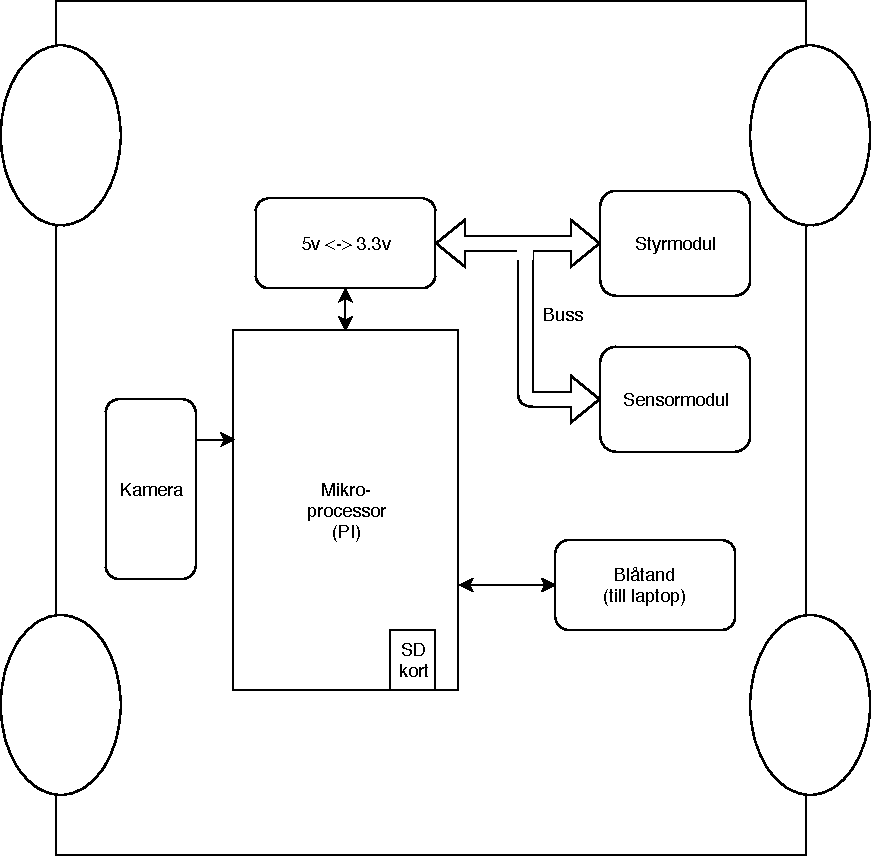
\includegraphics[width=0.6\linewidth]{systemskiss/figures/kommodul.pdf}
    \caption{Övergripande bild över komunikationsmodulen}
    \label{fig:komskiss}
\end{figure}

\end{document}

